\documentclass[11pt]{article}
\usepackage[utf8]{inputenc}
\usepackage[english]{babel}
\usepackage{amsmath}
\usepackage{graphicx}
\usepackage{float}
\usepackage{lipsum}
\usepackage{multicol}
\usepackage{xcolor}
\usepackage{tabularx}
\usepackage{booktabs}
\usepackage{hyperref}
\newcolumntype{Y}{>{\centering\arraybackslash}X}
\usepackage[left=2.00cm, right=2.00cm, top=2.00cm, bottom=2.00cm]{geometry}

\title{AN2DL Reports Template}

\begin{document}
    
    \begin{figure}[H]
        \raggedright
        
\includegraphics[scale=0.4]{polimi.png} \hfill 
\includegraphics[scale=0.3]{airlab.jpeg}
    \end{figure}
    
    \vspace{5mm}
    
    \begin{center}
        % Select between First and Second
        {\Large \textbf{AN2DL - First Homework Report}}\\
        \vspace{2mm}
        % Change with your Team Name
        {\Large \textbf{cortex\_collective}}\\
        \vspace{2mm}
        % Team Members Information
        {\large Camilla Cesana,}
        {\large Shayan Korki,}
        {\large Bahman Amirsardary,}
        {\large Marco Casagrande }\\
        \vspace{2mm}
        % Codabench Nicknames
        {camillacesana,}
        {shayankorkii,}
        {bahman75,}
        {marcocasagrande}\\
        \vspace{2mm}
        % Matriculation Numbers
        {252108,}
        {242161,}
        {Matricola3,}
        {259184}\\
        \vspace{5mm}
        \today
    \end{center}    
    \vspace{5mm}
    \begin{multicols}{2}
        \section{Introduction}
        The problem addressed in this project involves the \textit{multi-output categorical regression problem} of blood cell state classification from digital images. Specifically, it is a \textit{supervised multi-class classification problem}, where each image, provided in RGB format and with a resolution of 96x96 pixels, must be assigned to one of eight possible classes, each representing a specific functional state of the cell.\\ 
        The approach to solving the classification task was structured around systematic steps aimed at optimizing model performance and accuracy:
        \begin{itemize}
            \item \textbf{Data Analysis and Preprocessing:}
                The process began with a comprehensive exploration of the training dataset, aimed at analyzing the distribution of classes, examining image characteristics and detecting outliers.
            \item \textbf{Development of a Custom CNN Architecture:}
                A custom convolutional neural network (CNN) architecture was designed and implemented with the aim of creating a solution that would help deepen our understanding of the subject and optimize the classification process.
            \item \textbf{Fine-Tuning Using Pretrained Models:}
                To further improve the model's accuracy, transfer learning was employed by fine-tuning a pretrained model on the dataset.
        \end{itemize}
        
        \section{Problem Analysis}
        \textbf{Dataset characteristics}: 
            As shown in Figure 1, the dataset contains 13,759 images of blood cells divided in 8 classes with a not homogeneous distribution.
            \begin{figure}[H]
                \centering
                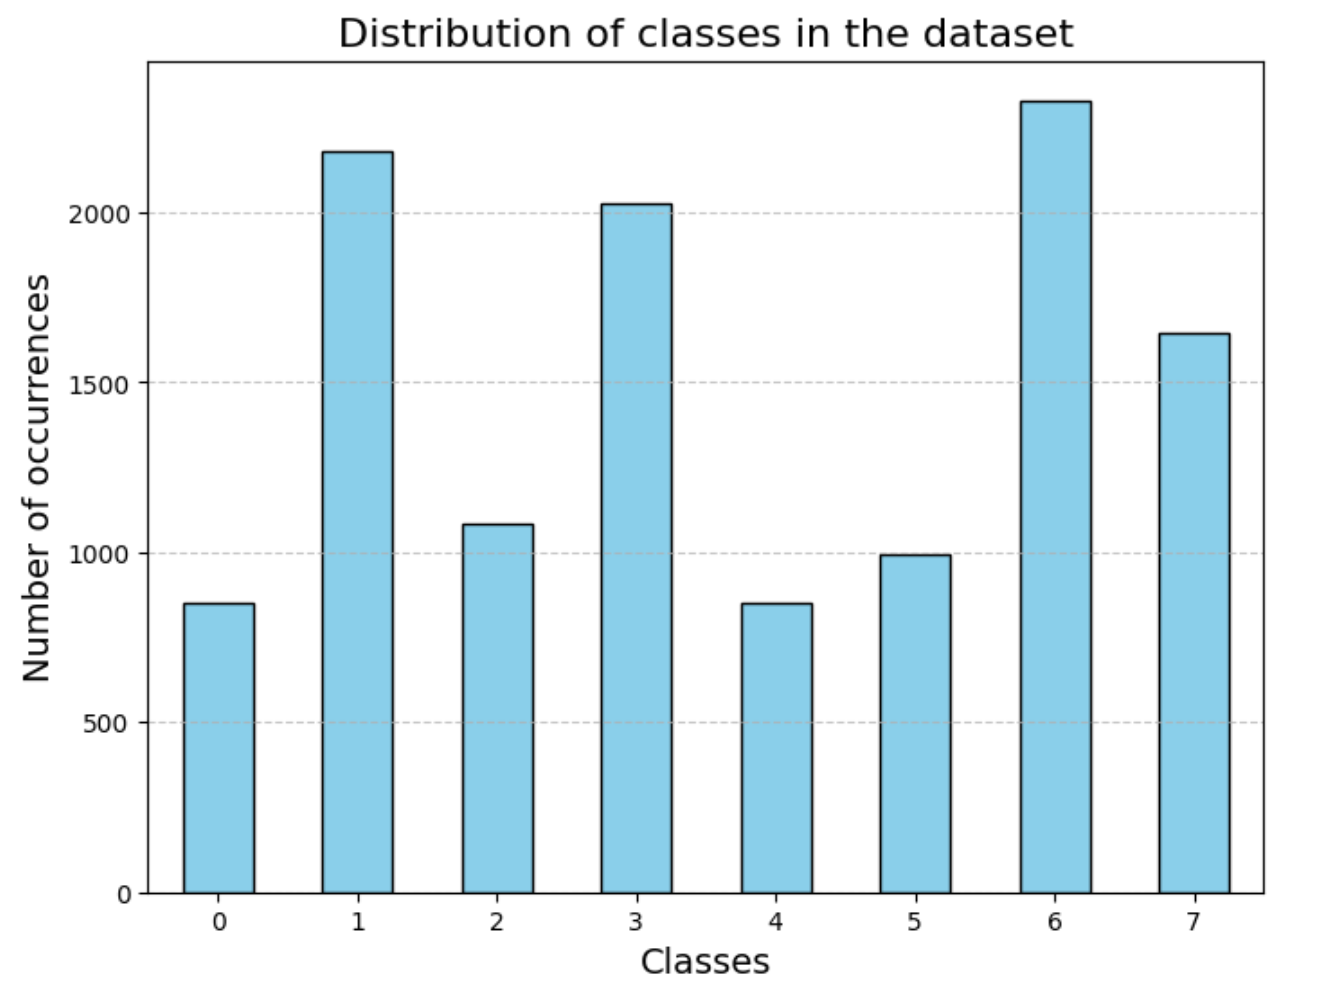
\includegraphics[width=0.75\linewidth]{classDistribution.png}
                \caption{Distribution of samples among the eight classes}
                \label{fig:results}
            \end{figure}
        \noindent \textbf{Main challenges}:
        During the dataset analysis, it was observed that two types of images included overlays with elements unrelated to the eight cell classes. Furthermore, these images were duplicated thousands of times, which could have negatively impacted the quality of the model's training.\\ \\
        An additional challenge lies in identifying a suitable convolutional neural network (CNN) model that can effectively and efficiently extract relevant features from the data. At the same time, it is crucial to ensure that the model does not overfit, as this could negatively impact its ability to generalize to new, unseen data. Striking the right balance between model complexity and generalization is key to achieving optimal performance.\\

        

        \noindent \textbf{Initial assumptions}: Due to the limited computational and storage resources in the development environment, it was not possible to train sufficiently deep custom convolutional neural networks. This imposed restrictions on the choice of model complexity, and as a result, it was necessary to start from pre-trained models using transfer learning.
       
        
       

        \section{Method}
        
        \textbf{Overview}: In this chapter, we will illustrate the methodologies used to address the main issues previously mentioned, divided into data and model. \\
        
        \noindent \textbf{Data:}
        \begin{itemize}
            \item \textbf{Dataset}: The dataset was preprocessed to eliminate images that were irrelevant to the input domain. To address the class imbalance, the SMOTE method from the imblearn.over\_sampling module was applied for oversampling reaching a target occurrence to 2330 images per class.
            \item \textbf{Data augmentation}: To improve the accuracy of the tested models, various data augmentation techniques were applied. In the initial phase, several transformations were introduced, including rotations, horizontal and vertical flips, spatial shifts, and adjustments to brightness and contrast. In a subsequent phase, a more advanced augmentation approach, called MixAug, was tested. This approach combines multiple geometric and photometric transformations synergistically. However, it did not lead to the desired improvements and, in fact, resulted in worse performance compared to the initial configuration.
            As a result, a strategy similar to the initial augmentation was adopted, with the addition of the Mixup technique that at batch level overlap two different images. This combination proved effective in enhancing the model's generalization ability, reducing the risk of overfitting, and improving overall robustness.
        \end{itemize}
        
        \noindent \textbf{Model}:
        The model selection process followed an incremental approach, starting with a simple self-designed neural network tailored to the task. We progressively modified the depth of the convolutional network, increased the number of parameters, adjusted filter dimensions, fine-tuned the size and number of hidden layers in the final stage, and optimized other hyperparameters. These adjustments led to continuous yet not decisive improvements. However, due to the platform limitations outlined in paragraph 2 and the evident need for a larger and more powerful model, given the unsatisfactory results obtained on the test set, we opted for transfer learning with fine-tuning.
        
        \section{Experiments}
         In this section are illustrated the descriptions and the results of the architectures designed.\\
        \textbf{Self-designed CNN}: The first CNN implemented \( (Custom\_1) \)  is based on a sequence of 4 blocks, each consisting of a convolutional layer with 3x3 kernel size and an incremental number of filters, a ReLU activation function and max pooling. Finally, a flattening layer is applied followed by the Dense Layer for the final classification. For this first version, we tried different techniques to improve performance such as dropout and GAP \( (Custom\_2) \).\\ Due to the very simple and shallow model, an additional convolutional layer was inserted between the first one and the pooling layer, inspired by the well-known VGG architecture \( (Custom\_3) \). This model was studied in conjunction with the oversampling technique and the elimination of inconsistent images from the database . 
        \\As a last model, following the idea of using known architectures, a structure was designed that presents the fundamentals of the ResNet model \( (Custom\_4) \) which concludes with the best test score of 0.31 \\
        The following table shows the performance on the validation set of the models described.
        \begin{table}[H]
            \centering
            \setlength{\tabcolsep}{3pt}
            \caption{Performance of self-designed models}
            \begin{tabularx}{\linewidth}{p{3.0cm} p{3.0cm} p{3.0cm}}
                \toprule
                Model & Val\_Accuracy & Val\_Loss\\
                \midrule
                Custom\_1 & 0.8699 & 0.3324\\
                Custom\_2 & 0.8063 & 0.6257\\
                Custom\_3 & 0.9345 & 0.1881\\
                Custom\_4 & 0.9496 & 0.1897\\
                \bottomrule
            \end{tabularx}
            \label{tb:Measurements}
        \end{table}


         \noindent\textbf{Transfer learning and fine-tuning CNN}: In the pursuit of continuity and rigor, the first pre-trained network tested was ResNet50. Several analyses and studies were conducted on it, mainly modulating the number of trainable parameters and the sensitivity (learning rate) with which these weights were modified, in order to seek the best results. The best-performing parameters involved freezing 100 layers, resulting in 19,481,960 trainable parameters, and a learning rate of 0.001. 
         \begin{table}[H]
            \centering
            \setlength{\tabcolsep}{3pt}
            \begin{tabularx}{\linewidth}{>{\centering\arraybackslash}p{1.9cm} >{\centering\arraybackslash}p{2.7cm} >{\centering\arraybackslash}p{1.8cm} >{\centering\arraybackslash}p{1.8cm}} 
                \toprule
                Model & Val\_Accuracy & Val\_Loss & Score\\
                \midrule
                ResNet50 & 0.9176 & 0.2476 & 0.44\\
                \bottomrule
            \end{tabularx}
            \label{tb:Measurements}
        \end{table}
        This model achieved an accuracy of 0.9179 and a loss of 0.2476 on the validation set. However, it only achieved a score of 0.44 on the test set.
        Ultimately, the model that achieved the best score, combined with all the previously mentioned augmentation techniques, was EfficientNetB6. With the right combination of trainable parameters and its moderate computational efficiency, it managed to obtain the best score on the test set.\\
        \noindent \textbf{Final CNN}:

        \section{Results}
        Present your main findings here. You might want to:
        \begin{itemize}
            \item Compare your results with baselines
            \item Highlight key achievements using \textbf{bold text}
            \item Explain any unexpected outcomes
        \end{itemize}

        \section{Discussion}
        In this section, analyse your results critically. Consider:
        \begin{itemize}
            \item Strengths and weaknesses
            \item Limitations and assumptions -> limitazioni della piattaforma di testing, importante a causa della grande diosparità tra trsining test e test set
        \end{itemize}

        \section{Conclusions}
        Summarise your work and discuss potential future directions. This is where you can:
        \begin{itemize}
            \item Restate main contributions
            \item Suggest improvements
            \item Propose future work
        \end{itemize}

        \bibliography{references}
        \bibliographystyle{abbrv}
    \end{multicols}
\end{document}